\documentclass[a4paper,11pt]{article}

\usepackage{fullpage}
\usepackage{color}
\usepackage{hyperref}
\usepackage{amsmath}
\usepackage{amssymb}
\usepackage{tikz}
\usepackage{tabularx}
\usepackage{booktabs}
\usepackage{amsmath}
\usepackage{multirow}
\usepackage{layouts}
\usepackage{array}
\usepackage{pgf}
\usepackage{tikz}

\usepackage{amssymb}
\usepackage{graphics}
\usepackage{fancyhdr}
\usepackage{eucal}
\usepackage{ifthen}
\usepackage{ifpdf}
\usepackage{lmodern}
\usepackage{amsthm}
\usepackage{catoptions} % For \Autoref


\usetikzlibrary{positioning}

\hypersetup{
  colorlinks,%
    citecolor=black,%
    filecolor=black,%
    linkcolor=black,%
    urlcolor=mygreylink     % can put red here to visualize the links
}

\newcommand{\Pred}[2]{\ensuremath{\mathtt{Predator}\left<#1, #2\right>}}
\newcommand{\Prey}[2]{\ensuremath{\mathtt{Prey}\left<#1, #2\right>}}
\newcommand{\p}[2]{\ensuremath{\mathtt{P_{11^2}}\left<#1, #2\right>}}
\newcommand{\pSW}[2]{\ensuremath{\mathtt{P_{6^2}}\left<#1, #2\right>}}
\newcommand{\pRSW}[2]{\ensuremath{\mathtt{P_{6^2}}\left<#1, #2\right>}}
\newcommand{\SN}[0]{\ensuremath{S_{11^4}}}
\newcommand{\SSW}[0]{\ensuremath{S_{6^2}}}
\newcommand{\SRSW}[0]{\ensuremath{S_{21}}}

\newcommand{\DrawSmallPred}[2]{\node at (A.center #1 #2) {$\pi$};}
\newcommand{\DrawSmallPrey}[2]{\node at (A.center #1 #2) {P};}
\newcommand{\DrawBigPred}[2]  {\node at (A.center #1 #2) {\Huge $\pi$};}
\newcommand{\DrawBigPrey}[2]  {\node at (A.center #1 #2) {\Huge P};}

\definecolor{hlcolor}{rgb}{1, 0, 0}
\definecolor{mygrey}{gray}{.85}
\definecolor{mygreylink}{gray}{.30}
\textheight=8.6in
\raggedbottom
\addtolength{\oddsidemargin}{-0.375in}
\addtolength{\evensidemargin}{0.375in}
\addtolength{\textwidth}{0.5in}
\addtolength{\topmargin}{-.375in}
\addtolength{\textheight}{0.75in}

\makeatletter
%% Provide \Autoref; the \autoref with a printed capital
\def\figureautorefname{figure}
\def\tableautorefname{table}
\def\partautorefname{part}
\def\appendixautorefname{appendix}
\def\equationautorefname{equation}
\def\AMSautorefname{equation}
\def\theoremautorefname{theorem}
\def\enumerationautorefname{case}
\def\Autoref#1{%
  \begingroup
  \edef\reserved@a{\cpttrimspaces{#1}}%
  \ifcsndefTF{r@#1}{%
    \xaftercsname{\expandafter\testreftype\@fourthoffive}
      {r@\reserved@a}.\\{#1}%
  }{%
    \ref{#1}%
  }%
  \endgroup
}
\def\testreftype#1.#2\\#3{%
  \ifcsndefTF{#1autorefname}{%
    \def\reserved@a##1##2\@nil{%
      \uppercase{\def\ref@name{##1}}%
      \csn@edef{#1autorefname}{\ref@name##2}%
      \autoref{#3}%
    }%
    \reserved@a#1\@nil
  }{%
    \autoref{#3}%
  }%
}

% For drawing grids
\pgfkeys{/pgf/grid lines/.initial=2}

\pgfdeclareshape{grid}{
    % inherit most things from the rectangle shape
    \inheritsavedanchors[from=rectangle]
    \inheritanchorborder[from=rectangle]
    \inheritanchor[from=rectangle]{center}
    \inheritanchor[from=rectangle]{north}
    \inheritanchor[from=rectangle]{south}
    \inheritanchor[from=rectangle]{west}
    \inheritanchor[from=rectangle]{east}
    \inheritanchor[from=rectangle]{south east}
    \inheritanchor[from=rectangle]{south west}
    \inheritanchor[from=rectangle]{north east}
    \inheritanchor[from=rectangle]{north west}
    \inheritbackgroundpath[from=rectangle]

    \savedmacro\lines{%
        \pgfmathtruncatemacro\lines{\pgfkeysvalueof{/pgf/grid lines}}%
    }

    % draw the grid
    \beforebackgroundpath{
        % store lower right in xa/ya and upper right in xb/yb
        \southwest \pgf@xa=\pgf@x \pgf@ya=\pgf@y
        \northeast \pgf@xb=\pgf@x \pgf@yb=\pgf@y

        % compute distance between the lines
        \pgfmathparse{(\the\pgf@xb-\the\pgf@xa)/(\lines + 1)}
        \pgf@xc=\pgfmathresult pt
        \pgfmathparse{(\the\pgf@yb-\the\pgf@ya)/(\lines + 1)}
        \pgf@yc=\pgfmathresult pt

        % draw grid
        \c@pgf@counta=0
        \c@pgf@countb\lines\relax
        \pgf@xb=\pgf@xa
        \advance\pgf@xb\pgf@xc\relax
        \pgfmathloop
            \ifnum\c@pgf@counta<\c@pgf@countb
                \pgfpathmoveto{\pgfpoint{\pgf@xb}{\pgf@ya}}
                \pgfpathlineto{\pgfpoint{\pgf@xb}{\pgf@yb}}
                \advance\c@pgf@counta 1\relax
                \advance\pgf@xb\pgf@xc\relax
        \repeatpgfmathloop
        % set \pgf@xb to the right side
        \c@pgf@counta=0
        \pgf@yb=\pgf@ya
        \advance\pgf@yb\pgf@yc\relax
        \pgfmathloop
            \ifnum\c@pgf@counta<\c@pgf@countb
                \pgfpathmoveto{\pgfpoint{\pgf@xa}{\pgf@yb}}
                \pgfpathlineto{\pgfpoint{\pgf@xb}{\pgf@yb}}
                \advance\c@pgf@counta 1\relax
                \advance\pgf@yb\pgf@yc\relax
        \repeatpgfmathloop
        \pgfusepath{stroke}
    }

    % add anchors for vertices (intersections of grid lines)
    % and center points (centers of the small rectangles).
    %
    % vertex anchors are simply called 'x y' with '0 0' being the lower left
    % vertex.
    % center anchors are called 'center x y' with 'center 1 1' being the center
    % of the lower left rectangle
    \pgfutil@g@addto@macro\pgf@sh@s@grid{%
        \c@pgf@counta\lines
        \advance\c@pgf@counta 1\relax
        \pgfmathloop\ifnum\c@pgf@counta>-1
            {% group to allow nesting of loops
                \c@pgf@countb\lines
                \advance\c@pgf@countb 1\relax
                \pgfmathloop\ifnum\c@pgf@countb>-1
                    \pgfutil@ifundefined{pgf@anchor@grid@\the\c@pgf@counta\space\the\c@pgf@countb}{%
                        % need to use xdef, so that \c@pgf@counta/b are expanded
                        % vertices
                        \expandafter\xdef\csname pgf@anchor@grid@\the\c@pgf@counta\space\the\c@pgf@countb\endcsname{%
                            \noexpand\southwest \noexpand\pgf@xa=\noexpand\pgf@x \noexpand\pgf@ya=\noexpand\pgf@y
                            \noexpand\northeast \noexpand\pgf@xb=\noexpand\pgf@x \noexpand\pgf@yb=\noexpand\pgf@y
                            \noexpand\pgfmathparse{(\noexpand\the\noexpand\pgf@xb-\noexpand\the\noexpand\pgf@xa)/(\noexpand\lines + 1)*\the\c@pgf@counta}
                            \noexpand\pgf@x=\noexpand\pgf@xa\noexpand\relax
                            \noexpand\advance\noexpand\pgf@x\noexpand\pgfmathresult pt\noexpand\relax
                            \noexpand\pgfmathparse{(\noexpand\the\noexpand\pgf@yb-\noexpand\the\noexpand\pgf@ya)/(\noexpand\lines + 1)*\the\c@pgf@countb}
                            \noexpand\pgf@y=\noexpand\pgf@ya\noexpand\relax
                            \noexpand\advance\noexpand\pgf@y\noexpand\pgfmathresult pt\noexpand\relax
                        }
                        % centers
                        \expandafter\xdef\csname pgf@anchor@grid@center\space\the\c@pgf@counta\space\the\c@pgf@countb\endcsname{%
                            \noexpand\southwest \noexpand\pgf@xa=\noexpand\pgf@x \noexpand\pgf@ya=\noexpand\pgf@y
                            \noexpand\northeast \noexpand\pgf@xb=\noexpand\pgf@x \noexpand\pgf@yb=\noexpand\pgf@y
                            \noexpand\pgfmathparse{(\noexpand\the\noexpand\pgf@xb-\noexpand\the\noexpand\pgf@xa)/(2*(\noexpand\lines + 1))*(2*\the\c@pgf@counta-1)}
                            \noexpand\pgf@x=\noexpand\pgf@xa\noexpand\relax
                            \noexpand\advance\noexpand\pgf@x\noexpand\pgfmathresult pt\noexpand\relax
                            \noexpand\pgfmathparse{(\noexpand\the\noexpand\pgf@yb-\noexpand\the\noexpand\pgf@ya)/(2*(\noexpand\lines + 1))*(2*\the\c@pgf@countb-1)}
                            \noexpand\pgf@y=\noexpand\pgf@ya\noexpand\relax
                            \noexpand\advance\noexpand\pgf@y\noexpand\pgfmathresult pt\noexpand\relax
                        }
                    }{\c@pgf@countb0\relax}
                    \advance\c@pgf@countb-1\relax
                \repeatpgfmathloop
            }
            \advance\c@pgf@counta-1\relax
        \repeatpgfmathloop
    }
}
\makeatother

\tikzset{smallgrid/.style={
            draw,
            grid,
            grid lines=10,
            minimum width=6cm,
            minimum height=6cm}
        }
\tikzset{biggrid/.style={
            draw,
            grid,
            grid lines=10,
            minimum width=15cm,
            minimum height=15cm}
        }
% End of code for grids

\newcommand{\resheading}[1]{{\large \colorbox{mygrey}{\begin{minipage}{\textwidth}{\textbf{#1 \vphantom{p\^{E}}}}\end{minipage}}}}

\newcommand{\mywebheader}{
  \begin{tabular}{@{}p{5in}p{4in}}
  {\resheading{Assignment 1: Single Agent Planning}} & {\Large 21 September, 2012}\\\vspace{0.2cm}
  \end{tabular}}

\begin{document}


\begin{center}
{\LARGE \textbf{Autonomous Agents}}\\ [1em]
\end{center}
\mywebheader

\begin{center}
{\Large By:} \\ \vspace{0.1cm}
{\Large Paris Mavromoustakos} \\  \vspace{0.1cm}
{\Large Georgios Methenitis} \\ \vspace{0.1cm}
{\Large Patrick de Kok} \\ \vspace{0.1cm}
{\Large Marios Tzakris}
\end{center}




\section*{Introduction}
The purpose of this first assignment was to implement a reinforcement learning task, of which the problem satisfies the Markov property.  Such a task is known as a Markov Decision Process (MDP).  To achieve this we used one prey, which is part of the environment and behaves in a known probabilistic way, and one agent, the predator, whose goal is to catch the prey.  When that happens the episode ends.  The environment we used is an 11 by 11 toroidal grid.  The task assumed that the entire MDP is known to our agent.  The agent could thus determine the optimal policy even before interacting with the environment.  

To implement the assignment we used the programming language Java.  The results are gathered from a laptop with a Intel Core 2 CPU with both cores running at 1.83 GHz.  The laptop has 2 GB of RAM memory.

\section*{Exercise 1}
In the first part, we simulated the environment while keeping the policies of the predator and the prey separate.  The environment has the ability to hold one or more predators and one or more prey.  The predator starts from position $\left<0,0\right>$ and the prey from $\left<5,5\right>$.  Both have an action set consisting of moving north, south, west, east, or staying stationary, respectively represented by the symbols $\uparrow$, $\downarrow$, $\leftarrow$, $\rightarrow$ and $\circ$. 

The predator choses one of these actions randomly, where each has an equal chance to be picked.  The prey choses $\circ$ with probability $0.8$, and the rest of the actions are equally probable chosen, with a probability of $0.05$.  However, if the prey directly ends up in the same area as the predator, that action is disabled.  In such a case, the probability for that action is set to $0$, and the other moving actions get a probability of $0.2 / 3 = 0.0\bar{6}$.

Each episode of the simulation ends when the predator catches the prey.  In the case that there are multiple prey and predators the episode ends when there is no living prey in the simulation environment.  In this first assignment we held all of our experiments with one predator and one prey.  In \autoref{tab:SimStat} we present the overall statistics for this part of the assignment.

\begin{table}[h!]
\caption{Statistics of the simulation where both the predator and prey move randomly.  The statistics are gathered over 100 runs.}
\label{tab:SimStat}
\begin{center}
\begin{small}
\begin{tabular}{|@{ }l@{ }@{ }l@{ }}
      Average steps: & 279.7 \\ 
      Max no. of steps: & 1350   \\ 
      Min no. of steps: & 22 \\ 
      Mean over 100 runs: & 279.7  \\ 
      Stdev over 100 runs: & 255.1 \\
    \end{tabular}      
\end{small}
\end{center}  
\end{table}

\section*{Exercise 2}
In order to evaluate the random policy we implemented Policy Evaluation, computing the state-value function $V^\pi(S)$ and determined the value for each state.  For every state $s \in S$, we iteratively compute
\begin{align*}
V^\pi{(S)} = \sum_{a}\pi(s,a)\sum_{s'}P_{ss'}^a[R_{ss'}^a + \gamma V^{\pi}(s')]
\end{align*}
This is done according the algorithm in Figure 4.1 of Sutton and Barto.

First, in the naive approach we computed the state-value function for every state in $\SN$.  After Policy Evaluation with $\gamma = 0.8$ has converged, we got the following state-value combinations:
\begin{align*}
  V^\pi(S)(\left\{\Pred{0}{0},\Prey{5}{5}\right\})   & = 0.0008 \\
    V^\pi(S)(\left\{\Pred{2}{3},\Prey{5}{4}\right\})   &= 0.8900 \\
    V^\pi(S)(\left\{\Pred{2}{10},\Prey{10}{0}\right\}) &= 0.8900 \\
    V^\pi(S)(\left\{\Pred{10}{10},\Prey{0}{0}\right\}) &= 0.8817
\end{align*}

We have also implemented Policy Evaluation for the reduced state spaces $\SSW$ and $\SRSW$.  The values for above states are for all state spaces the same.  However, we noticed that the algorithm runs significantly faster.  \Autoref{peap} presents the performance results we had performing this algorithm to smaller state spaces than the original one. We set the maximum error boundary ($\theta$ in the pseudocode) to zero in order to let our implementation produce more accurate results. This may cause an increase in our implementation's execution time.

\begin{table}[h!]
\caption{Policy Evaluation algorithm performance.}
\label{peap}
\begin{center}
\begin{tabular}{cccc}
\textbf{State Space} & \textbf{D. Factor} & \textbf{Iterations} & \textbf{Time of Execution (ms.)} \\
\midrule
$\SN$    & 0.9         & 202         & 245608 \\
        & 0.7         & 73        & 94660    \\
        & 0.5         & 46        & 57754    \\
        & 0.1         & 23        & 29467  \\
$\SSW$     & 0.9         & 215         & 821    \\
        & 0.7         & 72        & 369  \\
        & 0.5         & 44        & 283    \\
        & 0.1         & 16        & 114    \\
$\SRSW$      & 0.9         & 215         & 475  \\
        & 0.7         & 72        & 280  \\
        & 0.5         & 41        & 195  \\
        & 0.1         & 16        & 50  \\
\end{tabular}
\end{center}
\end{table}


\section*{Exercise 3}
When naively exploring the state space $S$, you will have to compute the value for all possible states, depending on four variables (the coordinates of both the predator and prey), each of which can have 11 different values.  This results in $11^4 = 14641$ different states.  Because of the toroidal structure of the world, the state $\left\{\Pred{x}{y}, \Prey{x'}{y'}\right\}$ is equivalent to $\left\{\Pred{x+a}{y+b}, \Prey{x'+a}{y'+b}\right\}$; there is no special square in the given world which has features that distinguish it from other squares.  From this follows that we can fix either $x, y$ or $x', y'$ to a certain value.  By doing so, we have removed two degrees of freedom, and reduced the space to only $11^2 = 121$ unique states.  Note that, when the position of the predator and prey are seen as vectors, this represents the difference vector $\Pred{x}{y} - \Prey{x'}{y'}$ or $\Prey{x'}{y'} - \Pred{x}{y}$, when respectively $x', y'$ or $x, y$ are fixed.  We have chosen to fix $x', y'$, and with $\p{x}{y}$ we denote the equivalence class of states for which $\left\{\Pred{x+a}{y+b}, \Prey{a}{b}\right\}$ holds.

For the means of computing $V(\cdot)$, we can shrink the state space even more.  Because of the symmetric nature of the world, the predator can catch the prey (and thus collect its reward) just as easily from any side.  This means that the following values correspond:
\begin{align*}
V(\pSW{x}{y})
  &= V(\p{x}{y}) \\
  &= V(\p{-x}{y}) \\
  &= V(\p{x}{-y}) \\
  &= V(\p{-x}{-y}) \\
  &= V(\p{x + 6 \lambda_1}{y + 6 \lambda_2}
\end{align*}

Through this, we only have to compute $V(\cdot)$ for $6^2 = 36$ different states.  The equivalent states under $\mathtt{P}_{6^2}$ are represented on an 11 by 11 grid in \autoref{fig:statespace6}.  The grid represents the space of $\mathtt{P}_{11^2}$.  A minimal, continuous area of this world is highlighted in red.

But even this representation contains symmetry.  This symmetry has its roots in the fact the predator likes to know best; how far away am I from the prey, when I move to this new spot?  Given $\p{x}{y}$, it can compute its Euclidean distance towards the prey $d(\p{x}{y}) = d(\pSW{x}{y}) = \sqrt{x^2+y^2}$.  For each move, it can recompute this distance, and based on this, it will assign a value.  There are only $\sum_{i=1}^{6} i = 21$ different distances, as the Euclidean distance is symmetrical in $x$ and $y$.  The equivalent states under $\mathtt{P}_{21}$ are represented on an 11 by 11 grid in \autoref{fig:statespace21}.  The grid represents the space of $\mathtt{P}_{11^2}$.  A minimal, continuous area of this world is highlighted in red.

We have implemented Policy Evaluation, Value Iteration and Policy Iteration for the naive, $11^4$-sized state space, for the square $6^2$-sized state space, and the triangular state space of $21$ states.  We refer to these spaces by $\SN$, $\SSW$ and $\SRSW$ respectively.

\begin{figure}
  \caption{Equivalent states under $\mathtt{P}_{6^2}$ are labeled with the same number.  The predator is assumed to be at $\left<0, 0\right>$.  The states indicate the position of the prey.  A single repetition of this set is highlighted in red.}
  \label{fig:statespace6}
\begin{center}
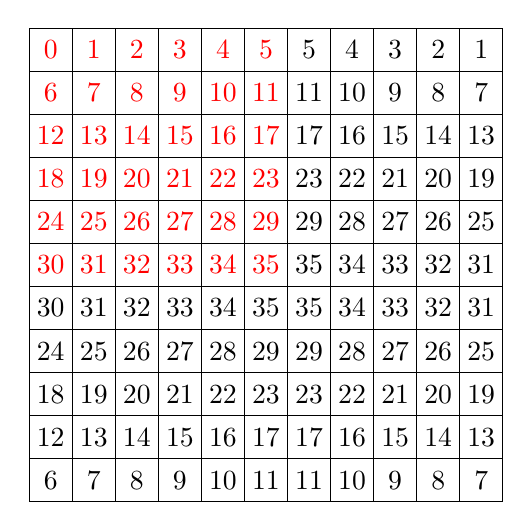
\begin{tikzpicture}
\node [smallgrid] (A) at (0,0) {};
\node[hlcolor] at (A.center 1  11) {0};
\node[hlcolor] at (A.center 2  11) {1};
\node[hlcolor] at (A.center 3  11) {2};
\node[hlcolor] at (A.center 4  11) {3};
\node[hlcolor] at (A.center 5  11) {4};
\node[hlcolor] at (A.center 6  11) {5};
\node at (A.center 7  11) {5};
\node at (A.center 8  11) {4};
\node at (A.center 9  11) {3};
\node at (A.center 10 11) {2};
\node at (A.center 11 11) {1};
\node[hlcolor] at (A.center 1  10) {6};
\node[hlcolor] at (A.center 2  10) {7};
\node[hlcolor] at (A.center 3  10) {8};
\node[hlcolor] at (A.center 4  10) {9};
\node[hlcolor] at (A.center 5  10) {10};
\node[hlcolor] at (A.center 6  10) {11};
\node at (A.center 7  10) {11};
\node at (A.center 8  10) {10};
\node at (A.center 9  10) {9};
\node at (A.center 10 10) {8};
\node at (A.center 11 10) {7};
\node[hlcolor] at (A.center 1  9) {12};
\node[hlcolor] at (A.center 2  9) {13};
\node[hlcolor] at (A.center 3  9) {14};
\node[hlcolor] at (A.center 4  9) {15};
\node[hlcolor] at (A.center 5  9) {16};
\node[hlcolor] at (A.center 6  9) {17};
\node at (A.center 7  9) {17};
\node at (A.center 8  9) {16};
\node at (A.center 9  9) {15};
\node at (A.center 10 9) {14};
\node at (A.center 11 9) {13};
\node[hlcolor] at (A.center 1  8) {18};
\node[hlcolor] at (A.center 2  8) {19};
\node[hlcolor] at (A.center 3  8) {20};
\node[hlcolor] at (A.center 4  8) {21};
\node[hlcolor] at (A.center 5  8) {22};
\node[hlcolor] at (A.center 6  8) {23};
\node at (A.center 7  8) {23};
\node at (A.center 8  8) {22};
\node at (A.center 9  8) {21};
\node at (A.center 10 8) {20};
\node at (A.center 11 8) {19};
\node[hlcolor] at (A.center 1  7) {24};
\node[hlcolor] at (A.center 2  7) {25};
\node[hlcolor] at (A.center 3  7) {26};
\node[hlcolor] at (A.center 4  7) {27};
\node[hlcolor] at (A.center 5  7) {28};
\node[hlcolor] at (A.center 6  7) {29};
\node at (A.center 7  7) {29};
\node at (A.center 8  7) {28};
\node at (A.center 9  7) {27};
\node at (A.center 10 7) {26};
\node at (A.center 11 7) {25};
\node[hlcolor] at (A.center 1  6) {30};
\node[hlcolor] at (A.center 2  6) {31};
\node[hlcolor] at (A.center 3  6) {32};
\node[hlcolor] at (A.center 4  6) {33};
\node[hlcolor] at (A.center 5  6) {34};
\node[hlcolor] at (A.center 6  6) {35};
\node at (A.center 7  6) {35};
\node at (A.center 8  6) {34};
\node at (A.center 9  6) {33};
\node at (A.center 10 6) {32};
\node at (A.center 11 6) {31};
\node at (A.center 1  5) {30};
\node at (A.center 2  5) {31};
\node at (A.center 3  5) {32};
\node at (A.center 4  5) {33};
\node at (A.center 5  5) {34};
\node at (A.center 6  5) {35};
\node at (A.center 7  5) {35};
\node at (A.center 8  5) {34};
\node at (A.center 9  5) {33};
\node at (A.center 10 5) {32};
\node at (A.center 11 5) {31};
\node at (A.center 1  4) {24};
\node at (A.center 2  4) {25};
\node at (A.center 3  4) {26};
\node at (A.center 4  4) {27};
\node at (A.center 5  4) {28};
\node at (A.center 6  4) {29};
\node at (A.center 7  4) {29};
\node at (A.center 8  4) {28};
\node at (A.center 9  4) {27};
\node at (A.center 10 4) {26};
\node at (A.center 11 4) {25};
\node at (A.center 1  3) {18};
\node at (A.center 2  3) {19};
\node at (A.center 3  3) {20};
\node at (A.center 4  3) {21};
\node at (A.center 5  3) {22};
\node at (A.center 6  3) {23};
\node at (A.center 7  3) {23};
\node at (A.center 8  3) {22};
\node at (A.center 9  3) {21};
\node at (A.center 10 3) {20};
\node at (A.center 11 3) {19};
\node at (A.center 1  2) {12};
\node at (A.center 2  2) {13};
\node at (A.center 3  2) {14};
\node at (A.center 4  2) {15};
\node at (A.center 5  2) {16};
\node at (A.center 6  2) {17};
\node at (A.center 7  2) {17};
\node at (A.center 8  2) {16};
\node at (A.center 9  2) {15};
\node at (A.center 10 2) {14};
\node at (A.center 11 2) {13};
\node at (A.center 1  1) {6};
\node at (A.center 2  1) {7};
\node at (A.center 3  1) {8};
\node at (A.center 4  1) {9};
\node at (A.center 5  1) {10};
\node at (A.center 6  1) {11};
\node at (A.center 7  1) {11};
\node at (A.center 8  1) {10};
\node at (A.center 9  1) {9};
\node at (A.center 10 1) {8};
\node at (A.center 11 1) {7};
\end{tikzpicture}
\end{center}
\end{figure}

\begin{figure}
  \caption{Equivalent states under $\mathtt{P}_{21}$ are labeled with the same number.  The predator is assumed to be at $\left<0, 0\right>$.  The states indicate the position of the prey.  A single repetition of this set is highlighted in red.}
  \label{fig:statespace21}
\begin{center}
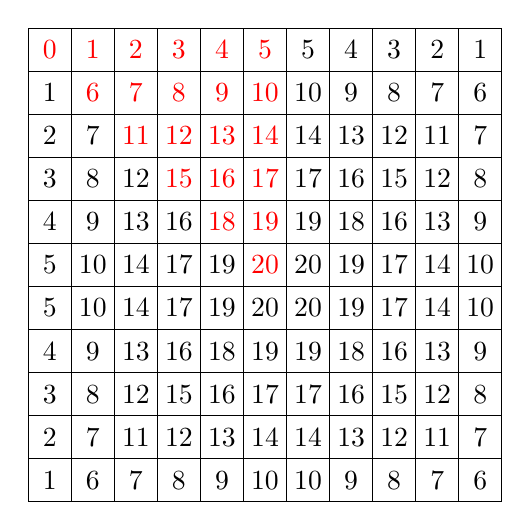
\begin{tikzpicture}
\node [smallgrid] (A) at (0,0) {};
\node[hlcolor] at (A.center 1  11) {0};
\node[hlcolor] at (A.center 2  11) {1};
\node[hlcolor] at (A.center 3  11) {2};
\node[hlcolor] at (A.center 4  11) {3};
\node[hlcolor] at (A.center 5  11) {4};
\node[hlcolor] at (A.center 6  11) {5};
\node at (A.center 7  11) {5};
\node at (A.center 8  11) {4};
\node at (A.center 9  11) {3};
\node at (A.center 10 11) {2};
\node at (A.center 11 11) {1};
\node at (A.center 1  10) {1};
\node[hlcolor] at (A.center 2  10) {6};
\node[hlcolor] at (A.center 3  10) {7};
\node[hlcolor] at (A.center 4  10) {8};
\node[hlcolor] at (A.center 5  10) {9};
\node[hlcolor] at (A.center 6  10) {10};
\node at (A.center 7  10) {10};
\node at (A.center 8  10) {9};
\node at (A.center 9  10) {8};
\node at (A.center 10 10) {7};
\node at (A.center 11 10) {6};
\node at (A.center 1  9) {2};
\node at (A.center 2  9) {7};
\node[hlcolor] at (A.center 3  9) {11};
\node[hlcolor] at (A.center 4  9) {12};
\node[hlcolor] at (A.center 5  9) {13};
\node[hlcolor] at (A.center 6  9) {14};
\node at (A.center 7  9) {14};
\node at (A.center 8  9) {13};
\node at (A.center 9  9) {12};
\node at (A.center 10 9) {11};
\node at (A.center 11 9) {7};
\node at (A.center 1  8) {3};
\node at (A.center 2  8) {8};
\node at (A.center 3  8) {12};
\node[hlcolor] at (A.center 4  8) {15};
\node[hlcolor] at (A.center 5  8) {16};
\node[hlcolor] at (A.center 6  8) {17};
\node at (A.center 7  8) {17};
\node at (A.center 8  8) {16};
\node at (A.center 9  8) {15};
\node at (A.center 10 8) {12};
\node at (A.center 11 8) {8};
\node at (A.center 1  7) {4};
\node at (A.center 2  7) {9};
\node at (A.center 3  7) {13};
\node at (A.center 4  7) {16};
\node[hlcolor] at (A.center 5  7) {18};
\node[hlcolor] at (A.center 6  7) {19};
\node at (A.center 7  7) {19};
\node at (A.center 8  7) {18};
\node at (A.center 9  7) {16};
\node at (A.center 10 7) {13};
\node at (A.center 11 7) {9};
\node at (A.center 1  6) {5};
\node at (A.center 2  6) {10};
\node at (A.center 3  6) {14};
\node at (A.center 4  6) {17};
\node at (A.center 5  6) {19};
\node[hlcolor] at (A.center 6  6) {20};
\node at (A.center 7  6) {20};
\node at (A.center 8  6) {19};
\node at (A.center 9  6) {17};
\node at (A.center 10 6) {14};
\node at (A.center 11 6) {10};
\node at (A.center 1  5) {5};
\node at (A.center 2  5) {10};
\node at (A.center 3  5) {14};
\node at (A.center 4  5) {17};
\node at (A.center 5  5) {19};
\node at (A.center 6  5) {20};
\node at (A.center 7  5) {20};
\node at (A.center 8  5) {19};
\node at (A.center 9  5) {17};
\node at (A.center 10 5) {14};
\node at (A.center 11 5) {10};
\node at (A.center 1  4) {4};
\node at (A.center 2  4) {9};
\node at (A.center 3  4) {13};
\node at (A.center 4  4) {16};
\node at (A.center 5  4) {18};
\node at (A.center 6  4) {19};
\node at (A.center 7  4) {19};
\node at (A.center 8  4) {18};
\node at (A.center 9  4) {16};
\node at (A.center 10 4) {13};
\node at (A.center 11 4) {9};
\node at (A.center 1  3) {3};
\node at (A.center 2  3) {8};
\node at (A.center 3  3) {12};
\node at (A.center 4  3) {15};
\node at (A.center 5  3) {16};
\node at (A.center 6  3) {17};
\node at (A.center 7  3) {17};
\node at (A.center 8  3) {16};
\node at (A.center 9  3) {15};
\node at (A.center 10 3) {12};
\node at (A.center 11 3) {8};
\node at (A.center 1  2) {2};
\node at (A.center 2  2) {7};
\node at (A.center 3  2) {11};
\node at (A.center 4  2) {12};
\node at (A.center 5  2) {13};
\node at (A.center 6  2) {14};
\node at (A.center 7  2) {14};
\node at (A.center 8  2) {13};
\node at (A.center 9  2) {12};
\node at (A.center 10 2) {11};
\node at (A.center 11 2) {7};
\node at (A.center 1  1) {1};
\node at (A.center 2  1) {6};
\node at (A.center 3  1) {7};
\node at (A.center 4  1) {8};
\node at (A.center 5  1) {9};
\node at (A.center 6  1) {10};
\node at (A.center 7  1) {10};
\node at (A.center 8  1) {9};
\node at (A.center 9  1) {8};
\node at (A.center 10 1) {7};
\node at (A.center 11 1) {6};
\end{tikzpicture}
\end{center}
\end{figure}


\section*{Exercise 4}
To find an optimal policy we computed the optimal value function $V^\ast$ for all states. First of all, we had to find the value function for the naive state space $\SN$. For all $s \in S$,
\begin{align*}
V^\pi(S) = \max_{a} \sum_{s'}P_{ss'}^a[R_{ss'}^a + \gamma V^{\pi}(s')]
\end{align*}
\Autoref{viat} presents the value table that was computed with the value iteration algorithm for a discount factor $\gamma = 0.7$ and $\theta = 0$. 
\begin{table}[h!]
\caption{The value function $V^\ast$ generated by Value Iteration, with the predator fixed at $\langle 5,5 \rangle$, discount factor $\gamma = 0.7$, and maximum error boundary $\theta = 0$.}
\label{viat}
\begin{center}
\begin{tabular}{|c|c|c|c|c|c|c|c|c|c|c|}
\hline
0.44 & 0.61 & 0.85 & 1.18 & 1.65 & 2.13 & 1.65 & 1.18 & 0.85 & 0.61 & 0.44 \\ \hline
0.61 & 0.84 & 1.18 & 1.67 & 2.35 & 3.09 & 2.35 & 1.67 & 1.18 & 0.84 & 0.61 \\ \hline
0.85 & 1.18 & 1.67 & 2.35 & 3.32 & 4.50 & 3.32 & 2.35 & 1.67 & 1.18 & 0.85 \\ \hline
1.18 & 1.67 & 2.35 & 3.32 & 4.69 & 6.55 & 4.69 & 3.32 & 2.35 & 1.67 & 1.18 \\ \hline
1.65 & 2.35 & 3.32 & 4.69 & 6.55 & 10.00 & 6.55 & 4.69 & 3.32 & 2.35 & 1.65 \\ \hline
2.13 & 3.09 & 4.50 & 6.55 & 10.00 & $\pi$ & 10.00 & 6.55 & 4.50 & 3.09 & 2.13 \\ \hline
1.65 & 2.35 & 3.32 & 4.69 & 6.55 & 10.00 & 6.55 & 4.69 & 3.32 & 2.35 & 1.65 \\ \hline
1.18 & 1.67 & 2.35 & 3.32 & 4.69 & 6.55 & 4.69 & 3.32 & 2.35 & 1.67 & 1.18 \\ \hline
0.85 & 1.18 & 1.67 & 2.35 & 3.32 & 4.50 & 3.32 & 2.35 & 1.67 & 1.18 & 0.85 \\ \hline
0.61 & 0.84 & 1.18 & 1.67 & 2.35 & 3.09 & 2.35 & 1.67 & 1.18 & 0.84 & 0.61 \\ \hline
0.44 & 0.61 & 0.85 & 1.18 & 1.65 & 2.13 & 1.65 & 1.18 & 0.85 & 0.61 & 0.44 \\ \hline
\end{tabular}
\end{center}
\end{table}
We also implemented the Value Iteration algorithm on the reduced state spaces $\SSW$ and $\SRSW$, acquiring the same values as above.  However, we noticed that the algorithm runs significantly faster.  \Autoref{viap} presents the performance results we had performing this algorithm to smaller state spaces than the original one.  We set $\theta$ variable to zero in order our algorithm to produce more accurate results.  This may cause an increase in the execution time of the Value Iteration algorithm.

\begin{table}[h!]
\caption{Value Iteration algorithm results. }
\label{viap}
\begin{center}
\begin{tabular}{cccc}
\textbf{State Space} & \textbf{D. Factor} & \textbf{Iterations} & \textbf{Time of Execution (ms.)} \\
\midrule
$\SN$ 		& 0.9 				& 29 				& 37774 \\
				& 0.7 				& 26 				& 34423 	 \\
 				& 0.5 				& 24 				& 31848 	 \\
 				& 0.1 				& 19 				& 24883  \vspace{0.1cm}  \\ 
$\SSW$			& 0.9 				& 22 				& 229 	 \\
				& 0.7 				& 19 				& 162  \\
				& 0.5 				& 16 				& 126 	 \\
				& 0.1 				& 11 				& 88 	 \vspace{0.1cm}  \\ 
$\SRSW$ 			& 0.9 				& 22 				& 93  \\
	 			& 0.7 				& 19 				& 70  \\
	 			& 0.5 				& 17 				& 67  \\
	 			& 0.1 				& 11 				& 60  \\
\end{tabular}
\end{center}
\end{table}

\section*{Exercise 5}
To iteratively improve the policy we implemented Policy Iteration $V^{\pi^\prime}$ for all states in all three state representations, $\SN$, $\SSW$ and $\SRSW$.  First, for all $s \in S$, we are doing a slightly modified version of Policy Evaluation.  After that, Policy Improvement is executed.  The procedure iterates with the same order until a stable policy for each state will be derived.  A policy is stable when, after a number of iterations of this algorithm, the policy converges into one that is optimal and cannot be changed to the better.  This is implemented as presented in Figure 4.3 of Sutton and Barto.  \Autoref{tab:piap} presents the result we had with our implementation of Policy Iteration, for different values for discount factor $\gamma$.  The maximum error boundary $\theta$ was set at $0$.

\begin{table}
\caption{Policy Iteration algorithm performance.}
\label{tab:piap}
\begin{center}
\begin{tabular}{@{ }c@{ }@{ }c@{ }@{ }c@{ }@{ }c@{ }}
\textbf{State Space} & \textbf{D. Factor $\gamma$} & \textbf{Iterations}& \textbf{Execution Time (ms.)} \\
\midrule
$\SN$ & 0.9 & 9 & 356222 \\
     & 0.7 & 8 & 152240 \\
     & 0.5 & 7 & 103164 \\
     & 0.1 & 8 & 61771 \vspace{0.1cm}  \\
$\SSW$  & 0.9 & 7 & 6221 \\
     & 0.7 & 6 & 2010 \\
     & 0.5 & 6 & 1005 \\
     & 0.1 & 5 & 353 \vspace{0.1cm}  \\ 
$\SRSW$   & 0.9 & 5 & 3594 \\
     & 0.7 & 5 & 1134 \\
     & 0.5 & 5 & 581 \\
     & 0.1 & 5 & 202 \\      
\end{tabular}
\end{center}
\end{table}


\section*{Conclusion}
We have managed to reduce the state space from $11^4$ states which should be processed separately to $11^2$, $6^2$ and $\sum_{i=1}^6 i$ equivalence classes of states.  We have implemented Policy Evaluation, Value Iteration and Policy Iteration for three of the four state space representations $\SN$, $\SSW$ and $\SRSW$.  The runtime of all algorithms is heavily reduced by running on the smallest state space.

The algorithms provide all equivalent values for the value function, which is expected.  This produces the same optimal policy, when maximizing over the value function.
\end{document}

